\documentclass[conference]{IEEEtran}
\IEEEoverridecommandlockouts
% The preceding line is only needed to identify funding in
% the first footnote. If that is unneeded, please comment it
% out.
\usepackage{cite}
\usepackage{hyperref}
\usepackage{amsmath,amssymb,amsfonts}
\usepackage{algorithmic}
\usepackage{graphicx}
\usepackage{textcomp}
\usepackage{xcolor}
\usepackage{placeins}
\usepackage{titlesec}

\setcounter{secnumdepth}{4}



\def\BibTeX{{\rm B\kern-.05em{\sc i\kern-.025em
    b}\kern-.08em
    T\kern-.1667em\lower.7ex\hbox{E}\kern-.125emX}}
\begin{document}

\title{ Fire Detection With Erroneous Input Correction\\
        { \footnotesize ECGR 4105/5105 - Introduction to
        Machine Learning} }

\author{\IEEEauthorblockN{1\textsuperscript{st} Jaskin
Kabir} \IEEEauthorblockA{\textit{ECGR Student} \\
\textit{UNC Charlotte}\\
Charlotte, NC \\
jkabir@charlotte.edu}
\and
\IEEEauthorblockN{2\textsuperscript{nd} Axel Leon Vasquez}
\IEEEauthorblockA{\textit{ECGR Student} \\
\textit{UNC Charlotte}\\
Charlotte, NC \\
aleonvas@charlotte.edu}
\and
\IEEEauthorblockN{3\textsuperscript{rd} Matthew Anderson}
\IEEEauthorblockA{\textit{ECGR Student} \\
\textit{UNC Charlotte}\\
Charlotte, NC \\
mande137@charlotte.edu} }
\maketitle

\begin{abstract}
The accuracy of typical fire alarm systems is often limited
due to their reliance on single sensors with constrained
detection capabilities. Moreover, a sensor failure renders
the entire system ineffective, posing a critical risk. While
AI-based fire detectors have massively outperformed
traditional systems, little work has addressed handling
sensor failures. To address this challenge, we propose
\textbf{AlarmNet}, a robust fire detection system that
incorporates erroneous sensor data during training. We
investigate two implementations of AlarmNet: a centralized
model trained on a single server and a simulation of a
federated model where training is distributed across
multiple clients and aggregated into a global model. In our
experiments, sensor errors were introduced by randomly
replacing 24.2\% of the dataset’s measurements with missing
or faulty values. We applied a pre-processing step that
replaced these values with the median of the corresponding
training features. Our 3-layer artificial neural network The
model achieved an accuracy of 98.38\% and successfully
detected 99.73\% of fires, despite the high rate of sensor
errors. This resulted in only a 0.25\% reduction in
detection performance compared to a model trained on
complete data, and a significant 41.51\% improvement over a
simulated commercial-grade fire alarm system." The federated
approach delivered comparable results while utilizing a less
computationally intensive model. In future work, we aim to
extend this approach to develop a real-world fire detection
system capable of maintaining robustness against sensor
failures.
\end{abstract}

\begin{IEEEkeywords}
machine learning (ML), algorithm, model, Artificial Neural
Network, Imputation, Sensor fusion, Fire Alarms, Fire
Detection, Error Handling, Federated Learning
\end{IEEEkeywords}

\section{Introduction and Motivation}\label{intro} 

Fire alarm systems play a critical role in safeguarding
lives and property by providing early warnings of fire
hazards. Traditional systems, however, do not perform as
well as their critical role would suggest. For example, a
2013 study found the Honeywell FS90, a widely used
commercial fire detection system, only achieves an accuracy
of 87.5\%\cite{smokeacc}. This contributes to deaths,
injuries, and damage due to fires in two ways. (1) When a
fire occurs and the fire detection system fails to recognize
it, the occupants of the building can only react to the fire
once they are close enough to observe it, often once it is
too late to evacuate. (2) A 1995 report stated that fewer
than 25\% of people interpreted the sound of the fire alarm
as a potential indication of a real emergency\cite{crywolf}.
Due to the high frequency of false or 'nuisance' alarms,
occupants may not evacuate or contact emergency services,
even if the alarm is triggered by a real fire.

As these systems typically rely on just one or two sensors
and simple logic to detect fires, they are especially
susceptible to faulty sensors rendering them completely
ineffective. While artificial intelligence (AI)-based fire
detectors have demonstrated significant improvements in
accuracy over traditional systems, they generally rely on
error-free sensor data\cite{ai1}\cite{ai2}\cite{ai3}. This
limits their practical applicability, especially in
real-world scenarios wherein sensor errors and failures are
common.

To address these challenges, we propose AlarmNet, a robust,
AI-based fire detection system specifically engineered to
remain accurate in the presence of sensor errors. AlarmNet
is trained on a dataset from which randomly selected
measurements were removed to simulate missing or faulty
sensor readings. This approach enables the model to learn to
detect fires accurately based on unreliable sensor data. 

The system is evaluated in two configurations: a centralized
model trained on a single server and a simulation of a
federated model, where training is distributed across
multiple clients and aggregated into a global model. This
dual approach allows us to investigate two key questions:
(1) whether it is possible to train a model that can handle
sensor errors, and (2) whether a federated model can achieve
comparable performance while utilizing fewer computational
resources. If the federated model meets this goal, it would
demonstrate AlarmNet's viability as a real-world fire
detection system. This paper first details the analysis and
preparation of the chosen dataset, followed by a disussion
of the design, implementation, and evaluation of both
versions of AlarmNet.

\section{Approach}

\section{Data Preparation}
\subsection{Dataset}
The dataset used in this project is the Smoke Detection
Dataset provided by Stefan Blattmann\cite{dataset}. The
dataset consists of approximately 62,629 sensor readings
encompassing both normal and fire-related scenarios,
providing diverse training and evaluating fire detection
models.

To generate this data, Blattman constructed an
Arduiono-based system to collect data from an array of six
sensors at a 1Hz sampling rate. These sensors were:
\begin{itemize}
    \item Bosch BMP390: Pressure Sensor
    \item Bosch BME688: Humidity, Temperature, and Gas
    Sensor (Volatile Organic Compounds/VOC)
    \item Bosch BMP388: Pressure Sensor
    \item Sensirion SPS30: Particular Matter Sensor
    \item Sensirion SHT31: Humidity and Temperature Sensor
    \item Sensirion SPG30: Gas sensor (VOC)
\end{itemize}
Note that several sensors measure the same environmental
factors, such as humidity and pressure. This redundancy is
intentional and serves to enhance the robustness of the
model. Before uploading this dataset to Kaggle, Blattman
utilized sensor fusion to combine the data from these six
sensors into a single dataset. The only sensor with no
redundancy is the Sensirion SPS30, which measures
particulate matter and is the most expensive sensor.

Blattman placed his sensor array into various fire scenarios
and recorded the measurements. He provided the following
short list of scenarios during which he collected data:
\begin{itemize}
    \item Normal indoor
    \item Normal outdoor
    \item Indoor wood fire, firefighter training area
    \item Indoor gas fire, firefighter training area
    \item Outdoor wood, coal, and gas grill
    \item Outdoor high humidity
    \item etc.
\end{itemize}
\cite{Blattmann}

\subsection{Train/Test Split}
Before the dataset was passed to the models, it was split
using an 80/20 train/test split. This means that 80\% of the
data were randomly sampled and used to train the model,
while the remaining 20\% were used to evaluate the model's
performance. This split ensures that the model is not
overfitting to the training data, as it is evaluated on data
that it has not seen before.

\subsection{Feature Scaling}
After the train/test split, the features were scaled using
standard scaling. This method subtracts the mean of the
feature and divides by the standard deviation, ensuring that
all features have a mean of 0 and a standard deviation of 1.
This scaling is important because it ensures that the model
does not learn to prioritize features with larger values,
which could lead to poor generalization. The mean and
standard deviation are calculated based on the training data
and then applied to the test data to ensure that the model
is evaluated on the same scale that it was trained on.

\subsection{Feature Elimination}
The dataset provided by Blattman originally included 15
features, which are listed in Table \ref{tab:features}. Of
these 15, the two sample count features and the timestamp
were removed as they do not provide any useful information
for the model. Of the remaining 12 features, a crucial task
was to determine which features were the most relevant to
the target variable. Eliminating irrelevant variables
reduces the complexity and computational cost of the model,
as its input space shrinks in dimensionality. This reduction
can also help prevent overfitting, as the model is less
likely to learn noise in the data.

\begin{table}[ht]
    \begingroup
    \renewcommand{\arraystretch}{1.5} % 
    \begin{tabular}{|p{0.25\linewidth}|p{0.65\linewidth}|}
        \hline
        \textbf{Feature} & \textbf{Description} \\
        \hline
        Timestamp & UTC Timestamp of the sample \\
        \hline
        Number & Unique identifier for each sample \\
        \hline
        Unnamed: 0 & Unintended duplicate of Number \\
        \hline
        Temperature & Air temperature in degrees Celsius \\
        \hline
        Humidity & Air humidity in percentage \\
        \hline
        Pressure & Air pressure in hectoPascals \\
        \hline
        TVOC & Total Volatile Organic Compounds in parts per
        billion \\
        \hline
        eC02 & Carbon Dioxide in parts per million \\
        \hline
        Raw H2 & Raw, uncompensated molecular hydrogen \\
        \hline
        Raw Ethanol & Raw, uncompensated ethanol \\
        \hline
        PM1.0 & Percentage of particles in the air less than
        1.0$\mu m$ in diameter \\
        \hline
        PM2.5 & Percentage of particles in the air less than
        2.5$\mu m$ in diameter \\
        \hline
        NC0.5 & Number concentration of particles in the air
        greater than 0.5$\mu m$ in diameter \\
        \hline
        NC1.0 & Number concentration of particles in the air
        greater than 1.0$\mu m$ in diameter \\
        \hline
        NC2.5 & Number concentration of particles in the air
        greater than 2.5$\mu m$ in diameter \\
        \hline
    \end{tabular}
    \vspace{1pt}
    \caption{Smoke Detection Dataset Features}
    \label{tab:features}
    \endgroup
\end{table}

To achieve this, we calculated the absolute correlation of
each feature with the target variable, 'Fire Alarm'. The
features were then ranked based on this correlation, and the
top four features were selected for the model. This number
was chosen by incrementally removing the least correlated
features from the dataset and training a model on the these
data until a significant drop in accuracy was measured.
These top four features were:
\begin{enumerate}
    \item Humidity
    \item Raw Ethanol
    \item Pressure
    \item TVOC
\end{enumerate}
While a sufficiently accurate model could be trained on
these data, this list of features does not include any of
the particulate matter measurements. If this system were to
ignore one of its sensors, it would be significantly less
resilient against sensor errors. To address this, we added
back the NC0.5 feature to the data, as it is the most
correlated with the target variable among the particulate
matter measurements.

\subsection{Error Insertion}
To simulate sensor errors, we developed a method to randomly
remove certain measurements from the dataset according to
some assumed rate of error. This rate of error represents
the chance that a given sensor reading will provide
incorrect or missing data during any given sample. We chose
to assume this error rate to be 40\%. This is an
unrealistically high number, but it is low enough to ensure
that the model is not completely useless while still
providing a significant challenge. 

Most of the features--with the exception of the particulate
matter measurements--were collected using two sensors. To
include this redundancy in the simulation, we assumed that
both sensors that generate any feature would have to fail
simultaneously in order for that feature to be missing for a
given a sample. In other words, while 40\% of the
particulate matter measurements were removed, only
20\%\footnote{The joint probability formula $P(A\cap
B=P(A)\times P(B))$ implies that this probability should
actually be 16\%. We chose to use 20\% instead for the added
challenge.} of the other measurements were removed. After
applying this error simulation to the dataset, approximately
24.2\% of the data was removed.

\subsection{Imputation}
Before this data could be used to train a model, the missing
values had to be replaced. We chose to use median
imputation, which replaces missing values with the median of
the corresponding feature calculated from the training
dataset. This method was chosen because it is robust to
outliers and skewed distributions, which are common in
sensor data.



\section{Model Training and Evaluation}

\subsection{Evaluation Methods}
\subsubsection{Multiple Models}
To ensure that the techniques used in this project are
effective, we trained and evaluated multiple models. We
trained a model based on the full 12-features of the
dataset, a model based on the top 4 features, a model that
included the NC0.5 feature for redundancy. We then compared
the performance of these three models to determine if the
feature elimination was necessary, and how adding back the
NC0.5 feature affected this performance.

We also trained a fully connected model on the imputed error
data, and a simulation of a federated learning system. The
performance of the federated model was then compared to the
fully connected model.
\subsubsection{Metrics}
The performance of each model was evaluated using the
following metrics:
\begin{itemize}
    \item Recall: Measures the proportion of actual fire
    cases detected by the model to minimize false negatives.
    This is the most important metric, as it is crucial that
    the model detects as many fires as possible.
    \begin{equation}
        \text{Recall} = \frac{\text{TP}}{\text{TP} + \text{FN}}
    \end{equation}
    \item Precision: The proportion of correctly identified
    fire alarms
    \begin{equation}
        \text{Precision} = \frac{\text{TP}}{\text{TP} + \text{FP}}
    \end{equation}
    \item F1-Score and Accuracy: Implements the harmonic
    mean of precision and recall with overall correctness of
    the model.
    \begin{equation}
        F1 = 2 \times \frac{\text{Precision} \times \text{Recall}}{\text{Precision} + \text{Recall}}
    \end{equation}
    \item Confusion Matrix: A visualization tool that lists
    the true positive/negative and false positive/negatives
\end{itemize}

\subsubsection{Honeywell FS90 Simulation}
The 2013 study mentioned in the introduction only listed the
Honeywell FS90's accuracy with no mention of precision,
recall, or the raw data necessary to calculate these values\cite{smokeacc}.
To provide a more accurate comparison, we developed a simple
simulation of the FS90:

First, we created a copy of the target column from the
training data. Then we randomly selected 12.5\% of the
datapoints in the data to flip, creating the FS90's 87.5\%
accurate 'prediction'. To simulate sensor error, we assumed
that the FS90 had a 20\% chance of experiencing a sensor
error during any given sample. This error rate was chosen to
match the rate of error in the AlarmNet model. We then
assumed that during a sensor error, the FS90 would indicate
that it did not detect a fire. To apply this to the
simulation, we randomly selected 20\% of the prediction
data. If the FS90 predicted a detected a fire during any of
these samples, we flipped the prediction to indicate that it
did not detect a fire. This simulation allowed us to
calculate the recall and precision of the FS90 with and
without sensor error, which we then compared to the AlarmNet
models.

\subsubsection{SVM Benchmark}
We trained a Support Vector Machine(SVM) on the same dataset as the model trained on the imputed error data. The SVM model was chosen as it was the best performing of the classical machine learning techniques on this dataset. The performance of this model was compared to the fully connected models to ensure that neural networks are the necessary for this application.

\subsection{Model Architectures}
For the model trained on the 12-feature model, the fully
connected neural network included an input layer of 12
neurons, two hidden layers of 64 and 32 neurons
respectively, and a layer consisting of one output neuron.
The 4 and 5-feature models used input layers of 4 and 5
neurons respectively, two hidden layers both consisting of
64 neurons, and one output neuron. Between each layer, a
ReLU activation function was used. This introduced
nonlinearity into the model, allowing it to learn complex
patterns in the data and ensuring its loss function was
differentiable. After the output layer, a sigmoid activation
function was applied to ensure that the output was between 0
and 1.

To allow the fully connected model trained on the data with
errors inserted into it, the architecture was increased to a
model with three hidden layers each consisting of 256
neurons. This allowed the model to learn more complex
patterns in the data and ensured that it could handle the
noisy and incomplete data.

The model used in the federated learning simulation used
three hidden layers consisting of 32, 16, and 8 neurons.
This model includes fewer neurons than any other model to
ensure that it is less computationally intensive. This model
was trained on three clients, each with a copy of the global
model. The clients trained their local models on their own
data, and then sent the weights of their models to the
global model. The global model then averaged these weights
to create a new global model.

\subsection{Training}
\subsubsection{Network Classes}
To train these models, we used the PyTorch library to develop the \texttt{AlarmNet} class. This class has a configurable number and size of hidden layers so that a new class doesn't have to be written for each network configuration. The class also includes methods to train the model, evaluate its performance, and generate visualizations of the model's performance. The class was then used to train the models on the training data and evaluate their performance on the test data.

Additionally, a \texttt{FederatedLearning} class was
developed to simulate the federated learning system. Upon
instantiation, this class instantiates a global instance of
the \texttt{AlarmNet} class. During training, it splits the
dataset into $n$ parts and then instantiates $n$ copies of
the global \texttt{AlarmNet} class to represent $n$
different clients. Each of these classes is then trained on
a different part of the dataset. After training, the weights
of each model are  averaged to update the global model. This
model is then evaluated on the test data to determine its
performance. $n$ is a configurable parameter, and so are the
number of training epochs each client trains for and how
many times this process is repeated.
\footnote{The code can be found at \url{https://github.com/jaskinkabir/Intro_ML_Project}}

\subsubsection{Training Parameters}
The models were trained using the Adam optimizer. The loss function used was binary cross-entropy, which is commonly used for binary classification problems. The models trained on the data without inserted errors used a learning rate of $10^{-3}$ and were trained for 3000 epochs. 

To accommodate the error model's larger architecture, the learning rate was reduced to $10^{-5}$ and the model was trained for 16000 epochs. 

The federated model was trained with a learning rate of $10^{-3}$ for the global model and the clients. We chose to simulate three clients, each performing 600 training epochs per round. The process of training the client models for 600 epochs and averaging their weights was repeated 3 times.

\section{Results and Analysis}
In a comparative analysis, SVM(Support Vector Machine) and
NN (Neural Network) were both considered for fire detection
within the 12-feature test bench. Neural networks are
ultimately chosen for their superior flexibility and
robustness. SVMs are known for their simplicity and
effectiveness within smaller datasets due to their ability
to model linear and non-linear relationships using kernel
functions. However, in this dataset, the project had a large
size of 62,000 samples which limited the SVM training model
as memory requirement scale quadratically with the number of
samples. On the other hand neural network demonstrates
superior performance and adaptability. They efficiently
scaled with large datasets by leveraging batch size gradient
descent and GPU acceleration with mixed precision and
gradient scaling. It can learn hierarchical features
representing them as particularity effective for
multi-sensor data its architecture model is tailored to
handle noisy and missing data, as seen in the imputed error
model under results., It can maintain high recall and
precision under a 20 percent error rate. The full feature
model utilizes all 12 -features that achieved high precision
and recall but its computational complexity made it less
efficient. After using a correlation technique ranking them
by target variable it reduced to 4 and 5 feature sets
retaining only the top four features ( Humidity, Raw
Ethanol, Pressure, and TVOC), achieved performance to the
full feature model with minimal precision loss of 0.1
percent. It significantly improved making it more suitable
for different environments. The redundant feature model
added the NC0.5 enchanting redundancy and improved
robustness maintaining efficiency. The imputed error model
designed to handle noisy and missing data shows a resilience
with 20 percent error rate. Thus outperforming the Honeywell
FS90 system. In addition to accuracy and recall, time was
evaluated to determine real-time applicability. The proposed
models achieve an average time of 2e-2 seconds per sample
making them viable for deployment in fire detection systems.
Evaluation metrics showed visual comparison including
confusion matrices, and bar charts illustrating the superior
performance. The reduced features and imputed error and
aggregation demonstrated the ability to balance accuracy,
efficiency, and robustness for real-world fire detection
applications. The Federated model trains the local copy of a
global model using local data. The training sends model
weights (weights of the neurons in the neural network) to
the global mode. The federate and AlarmNet achieve near
identical accuracy. These bar graphs show the comparison of
recall with and without error and precision with 20 percent
error and without. With Machine Learning algorithms, it was
able to provide excellent validation against Honeywell FS90
highlighting the potential ANN that can provide for
enchanting better real-world safety protocols (fig 18 and
19). 

\section{Lessons Learned}
This machine learning model successfully demonstrated the
development an efficient fire detection system using sensor
data. By leveraging a custom neural network architecture,
the system achieved high precision and recall even with
real-world scenarios such as noisy or missing sensor data.
Feature selections and target preparation, including median
imputation and error handling, ensure the model's
exploration. The reduced feature model maintained comparable
performance to the 12-feature model significantly reducing
computational requirements and making it good for
constrained environments. Comparative analysis highlights
the proposed neural network over the traditional such as
SVM. The neural network can handle large datasets, capture
complex features tolerate sensor errors underscores the
effects in IoT-base fire detection systems. Optimizing time
and compact model size ensure viability for read-time
devices. The project object results emphasize the importance
of designing models that are balanced, efficient, accurate,
and robust for safety and critical protocol applications.
Future work can be explored further optimizing the learning,
advancing imputation, and improving the federated model
weights between three clients to enhance system performance.
The project demonstrates the potential for machine learning
to revolutionize fire detection technology to challenge
high-end companies such as Honeywell to ensure the power of
ANN to contribute to improving safety and reliability in
diverse environments.






\section{Contributions}
\begin{itemize}
\item\textbf{Matthew Anderson:} 
\begin{itemize}
    \item Federated Learning Class
    \item Edited Report and Presentation
\end{itemize}

\item\textbf{Jaskin Kabir:} 
\begin{itemize}
    \item Project Manager
    \item Dataset Selection, Preparation, and Analysis
    \item AlarmNet Class that contained the fully connected
    model
    \item Error insertion and imputation
    \item Edited Report and Presentation
\end{itemize}

\item\textbf{Axel Leon Vasquez:} 
\begin{itemize}
    \item Wrote Report
    \item Created Presentation
    \item Data Visualization
\end{itemize}
\end{itemize}
\subsection{References}

\bibliographystyle{IEEEtran}
\bibliography{refs.bib}



\subsection{Results} 

\begin{figure}
    \centering
    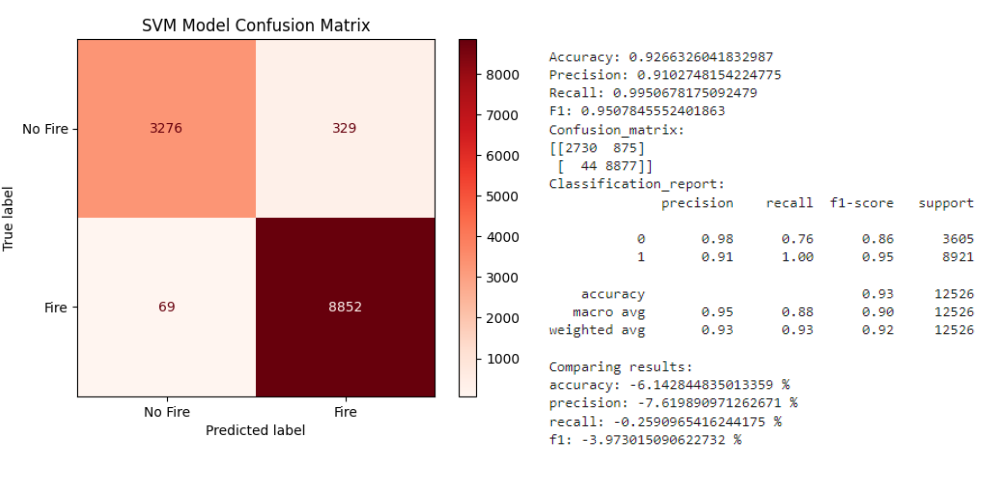
\includegraphics[width=0.75\linewidth]{images/SVM.png}
    \caption{SVM Metric}
    \label{fig: SVM Model}
\end{figure}

\begin{figure}
    \centering
    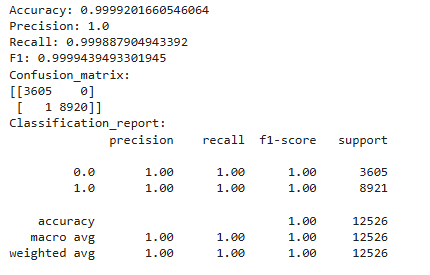
\includegraphics[width=0.75\linewidth]{images/12acc.png}
    \caption{12 - Feature Metrics}
    \label{fig: 1.0 }
\end{figure}

\begin{figure}
    \centering
    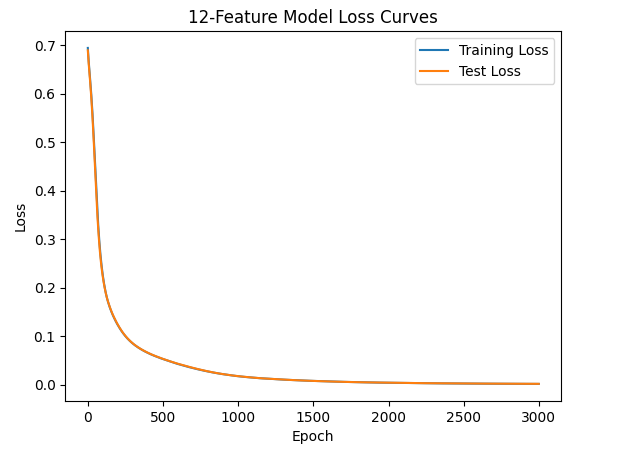
\includegraphics[width=0.75\linewidth]{images/12CM.png}
    \caption{12 - Feature Loss Curve}
    \label{fig: 1.2}
\end{figure}

\begin{figure}
    \centering
    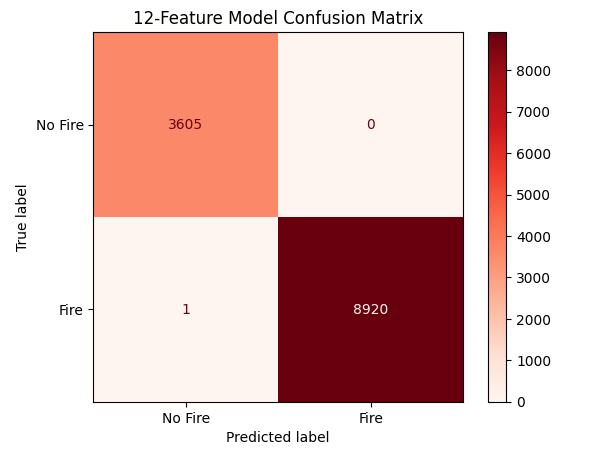
\includegraphics[width=0.75\linewidth]{images/12CMM.png}
    \caption{12 - Feature Confusion Matrix}
    \label{fig:1.3}
\end{figure}

\begin{figure}
    \centering
    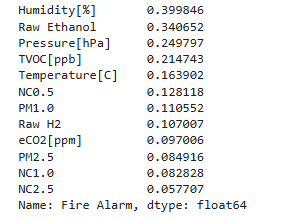
\includegraphics[width=0.7\linewidth]{images/Corr.png}
    \caption{Features}
    \label{fig:2.0-label}
\end{figure}

\begin{figure}
    \centering
    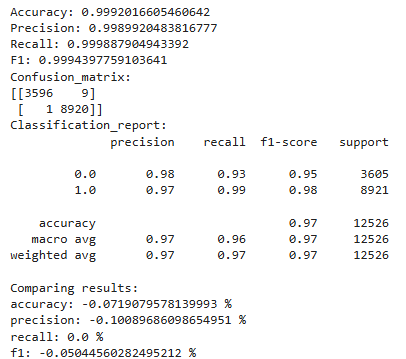
\includegraphics[width=0.75\linewidth]{images/4metric.png}
    \caption{4 - Feature Metrics}
    \label{fig:3.0}
\end{figure}

\begin{figure}
    \centering
    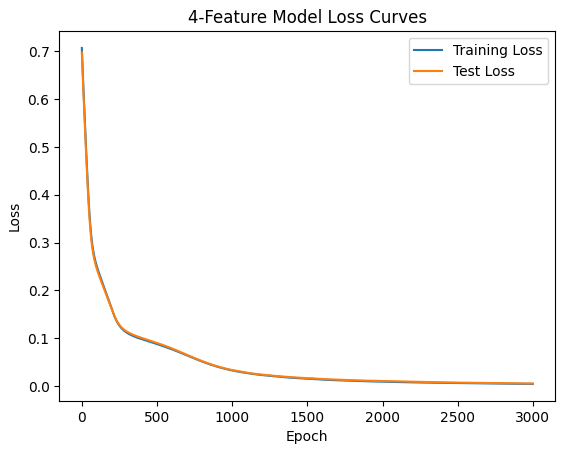
\includegraphics[width=0.75\linewidth]{images/4LC.png}
    \caption{4 - Feature Loss Curves}
    \label{fig:3.1}
\end{figure}

\begin{figure}
    \centering
    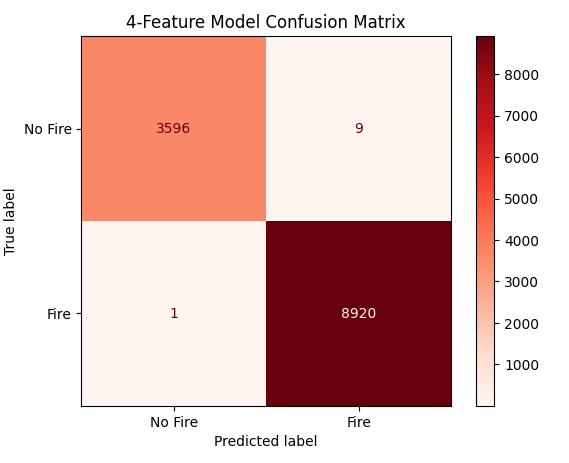
\includegraphics[width=0.75\linewidth]{images/4CM.png}
    \caption{4 - Feature Confusion Matrix}
    \label{fig:3.2}
\end{figure}

\begin{figure}
    \centering
    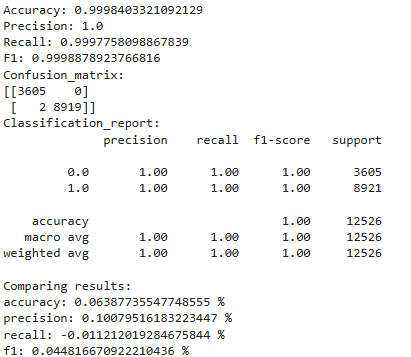
\includegraphics[width=0.75\linewidth]{images/5metric.png}
    \caption{5 - Feature Metrics}
    \label{fig:4.0}
\end{figure}

\begin{figure}
    \centering
    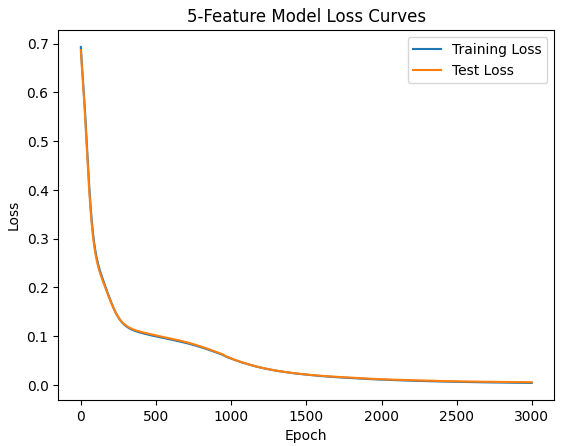
\includegraphics[width=0.75\linewidth]{images/5LC.png}
    \caption{5 - Feature Loss Curves}
    \label{fig:4.1}
\end{figure}

\begin{figure}
    \centering
    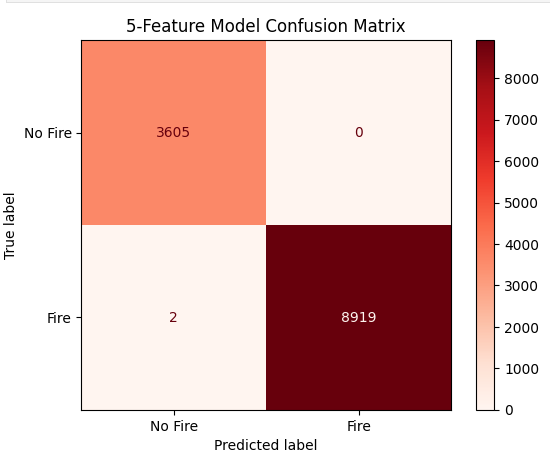
\includegraphics[width=0.75\linewidth]{images/5CM.png}
    \caption{5 - Feature Confusion Matrix}
    \label{fig:4.2}
\end{figure}

\begin{figure}
    \centering
    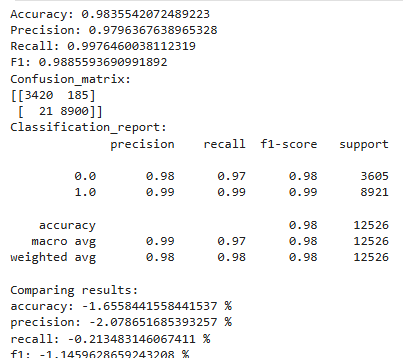
\includegraphics[width=0.75\linewidth]{images/imputationmetric.png}
    \caption{Imputation Metrics}
    \label{fig:5.0}
\end{figure}
\begin{figure}
    \centering
    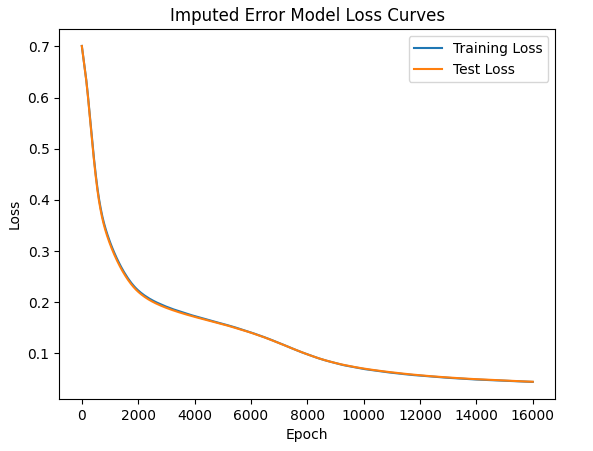
\includegraphics[width=0.75\linewidth]{images/ImputationLC.png}
    \caption{Imputation Loss Curves}
    \label{fig:5.1}
\end{figure}

\begin{figure}
    \centering
    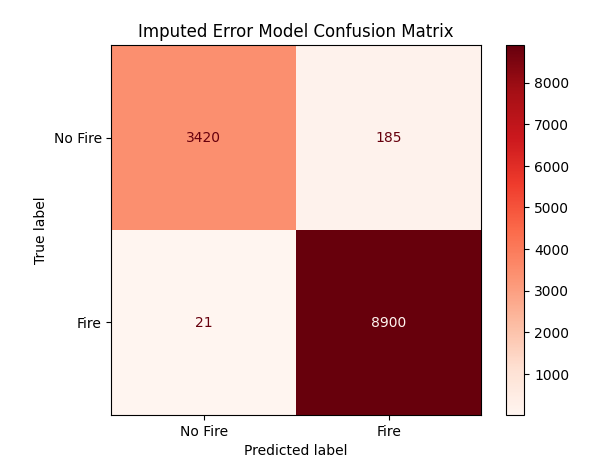
\includegraphics[width=0.75\linewidth]{images/ImputationCM.png}
    \caption{Imputation Confusion Matrix}
    \label{fig:5.2}
\end{figure}


\begin{figure}
    \centering
    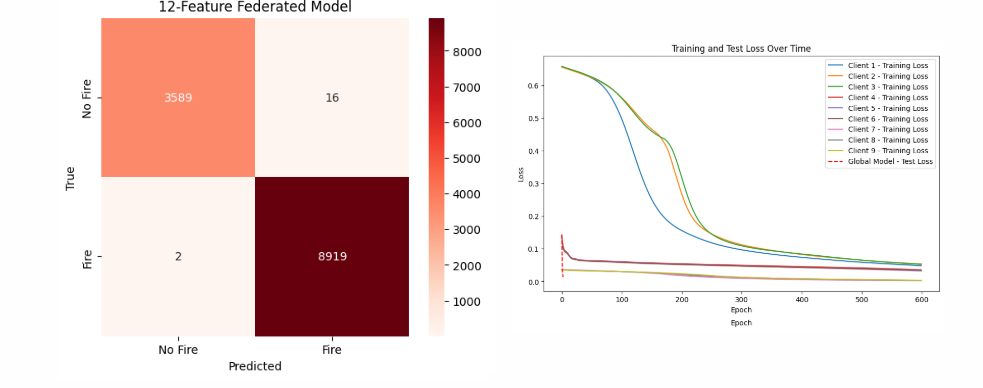
\includegraphics[width=1\linewidth]{images/12Fed.png}
    \caption{Federarted Learning: 12-Features}
    \label{fig:6.0}
\end{figure}

\begin{figure}
    \centering
    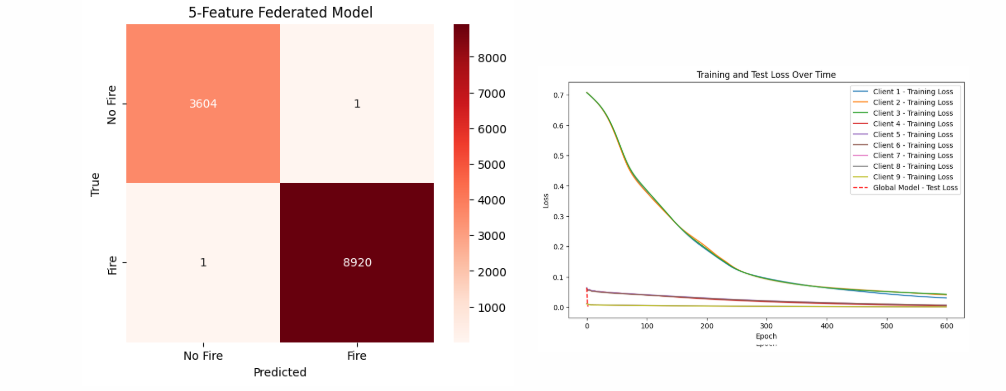
\includegraphics[width=1\linewidth]{images/5Fed.png}
    \caption{Federated Learning: 5-Features}
    \label{fig:6.1}
\end{figure}

\begin{figure}
    \centering
    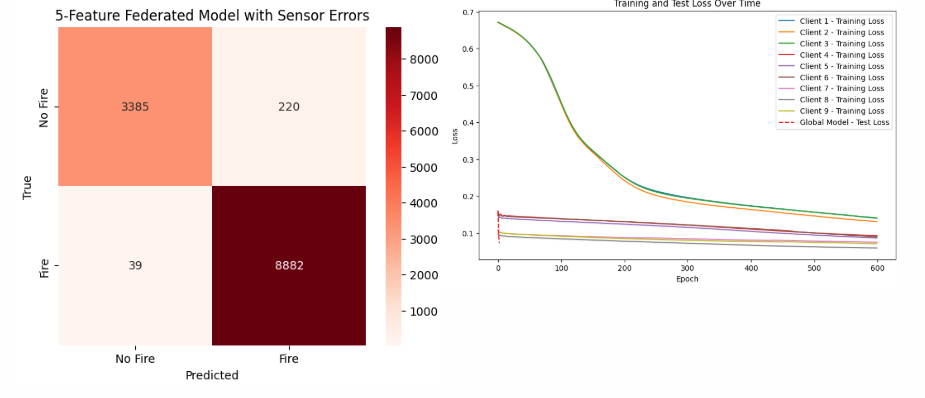
\includegraphics[width=1\linewidth]{images/FedHandling.png}
    \caption{Federated Learning: Error handling}
    \label{fig:6.2}
\end{figure}

\begin{figure}
    \centering
    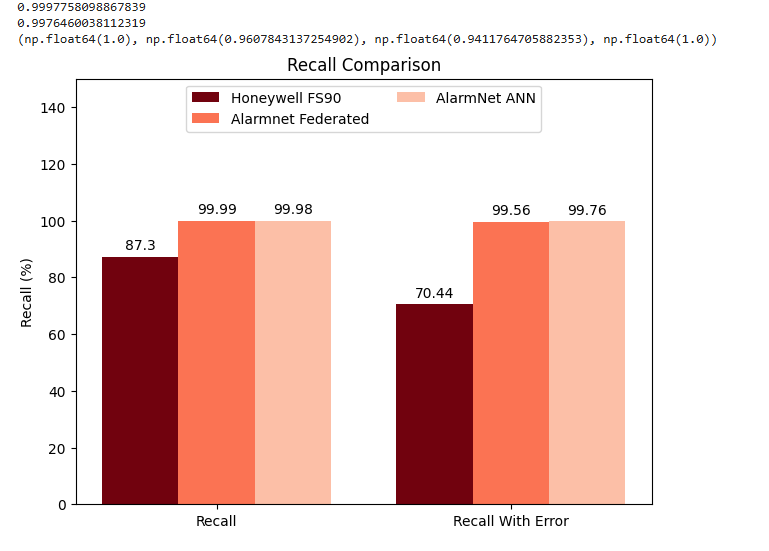
\includegraphics[width=0.75\linewidth]{images/Recall.png}
    \caption{Recall Comparison Honeywell FS90 Vs AlarmNet ANN Vs Federated}
    \label{fig:7.0}
\end{figure}

\begin{figure}
    \centering
    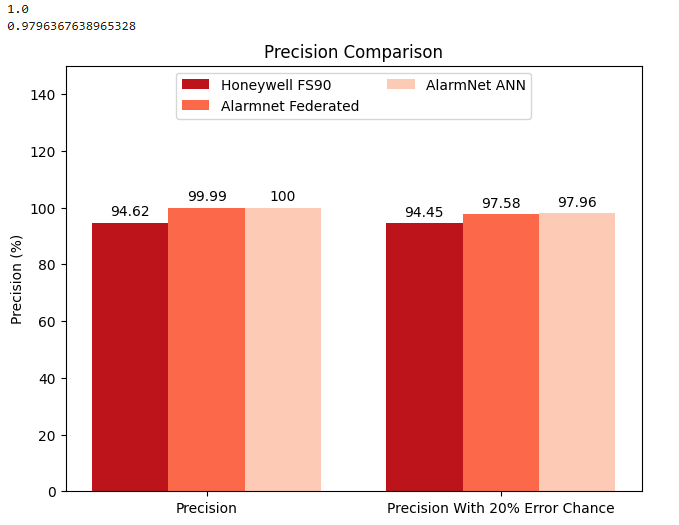
\includegraphics[width=0.75\linewidth]{images/PrecisionComparison.png}
    \caption{Precison Comparison Honeywell FS90 Vs AlarmNet ANN Vs Federated}
    \label{fig:7.1}
\end{figure}

\end{document}